\subsection{Información general del MCU}

El nRF52840 es el miembro más avanzado de la serie nRF52. Cumple con los desafíos de las aplicaciones sofisticadas que necesitan concurrencia de protocolos y un conjunto rico y variado de periféricos y funciones. Ofrece una generosa disponibilidad de memoria tanto para Flash como para RAM, que son requisitos previos para aplicaciones tan exigentes\cite{mcu}.
Se trata de un procesador ARM Cortex-M4 con unidad de coma flotante (FPU) que tiene un conjunto de instrucciones de 32 bits que implementa un superconjunto de instrucciones de 16 y 32 bits para maximizar la densidad del código y
actuación \cite{mcu}.\\
Tiene numerosos periféricos e interfaces digitales, como SPI y QSPI de alta velocidad para conectarse a pantallas y flashes externos, PDM e I2S para micrófonos y audio digitales, y un dispositivo USB de alta velocidad para transferencia de datos y fuente de alimentación para recargar la batería\cite{mcu}. A continuación en la tabla \ref{t1} se presenta las características eléctricas, en la figura \ref{f2} se presenta el diagrama de pines de la placa en donde se integra el MCU a utilizar, y en la figura \ref{f3} se presenta el diagrama de bloques. 


\begin{table}[H]
\centering
\begin{tabular}{|c|c|}
\hline
MCU                      & nRF52840             \\ \hline
Voltaje de operación     & 3.3V                             \\ \hline
Voltaje de entrada       & 21V                              \\ \hline
DC corriente por I/O Pin & 15 mA                            \\ \hline
Frecuencia de reloj      & 64MHz                            \\ \hline
Memoria Flash            & 1MB (nRF52840)                   \\ \hline
SRAM                     & 256KB (nRF52840)                 \\ \hline
EEPROM                   & none                             \\ \hline
I/O Digital Pins         & 14                               \\ \hline
PWM Pins                 & 14 (Todos los pines digitales)   \\ \hline
UART                     & 1                                \\ \hline
SPI                      & 1                                \\ \hline
I2C                      & 1                                \\ \hline
Analog Input Pins        & 8 (ADC 12 bit 200 ksamples)      \\ \hline
Analog Output Pins       & Only through PWM (no DAC)        \\ \hline
External Interrupts      & all digital pins                 \\ \hline
LED\_BUILTIN             & 13                               \\ \hline
USB                      & Native in the nRF52840 Processor \\ \hline

\end{tabular}
\caption{Características generales y eléctricas}
\label{t1}
\end{table}



\begin{figure}[H]
\centering
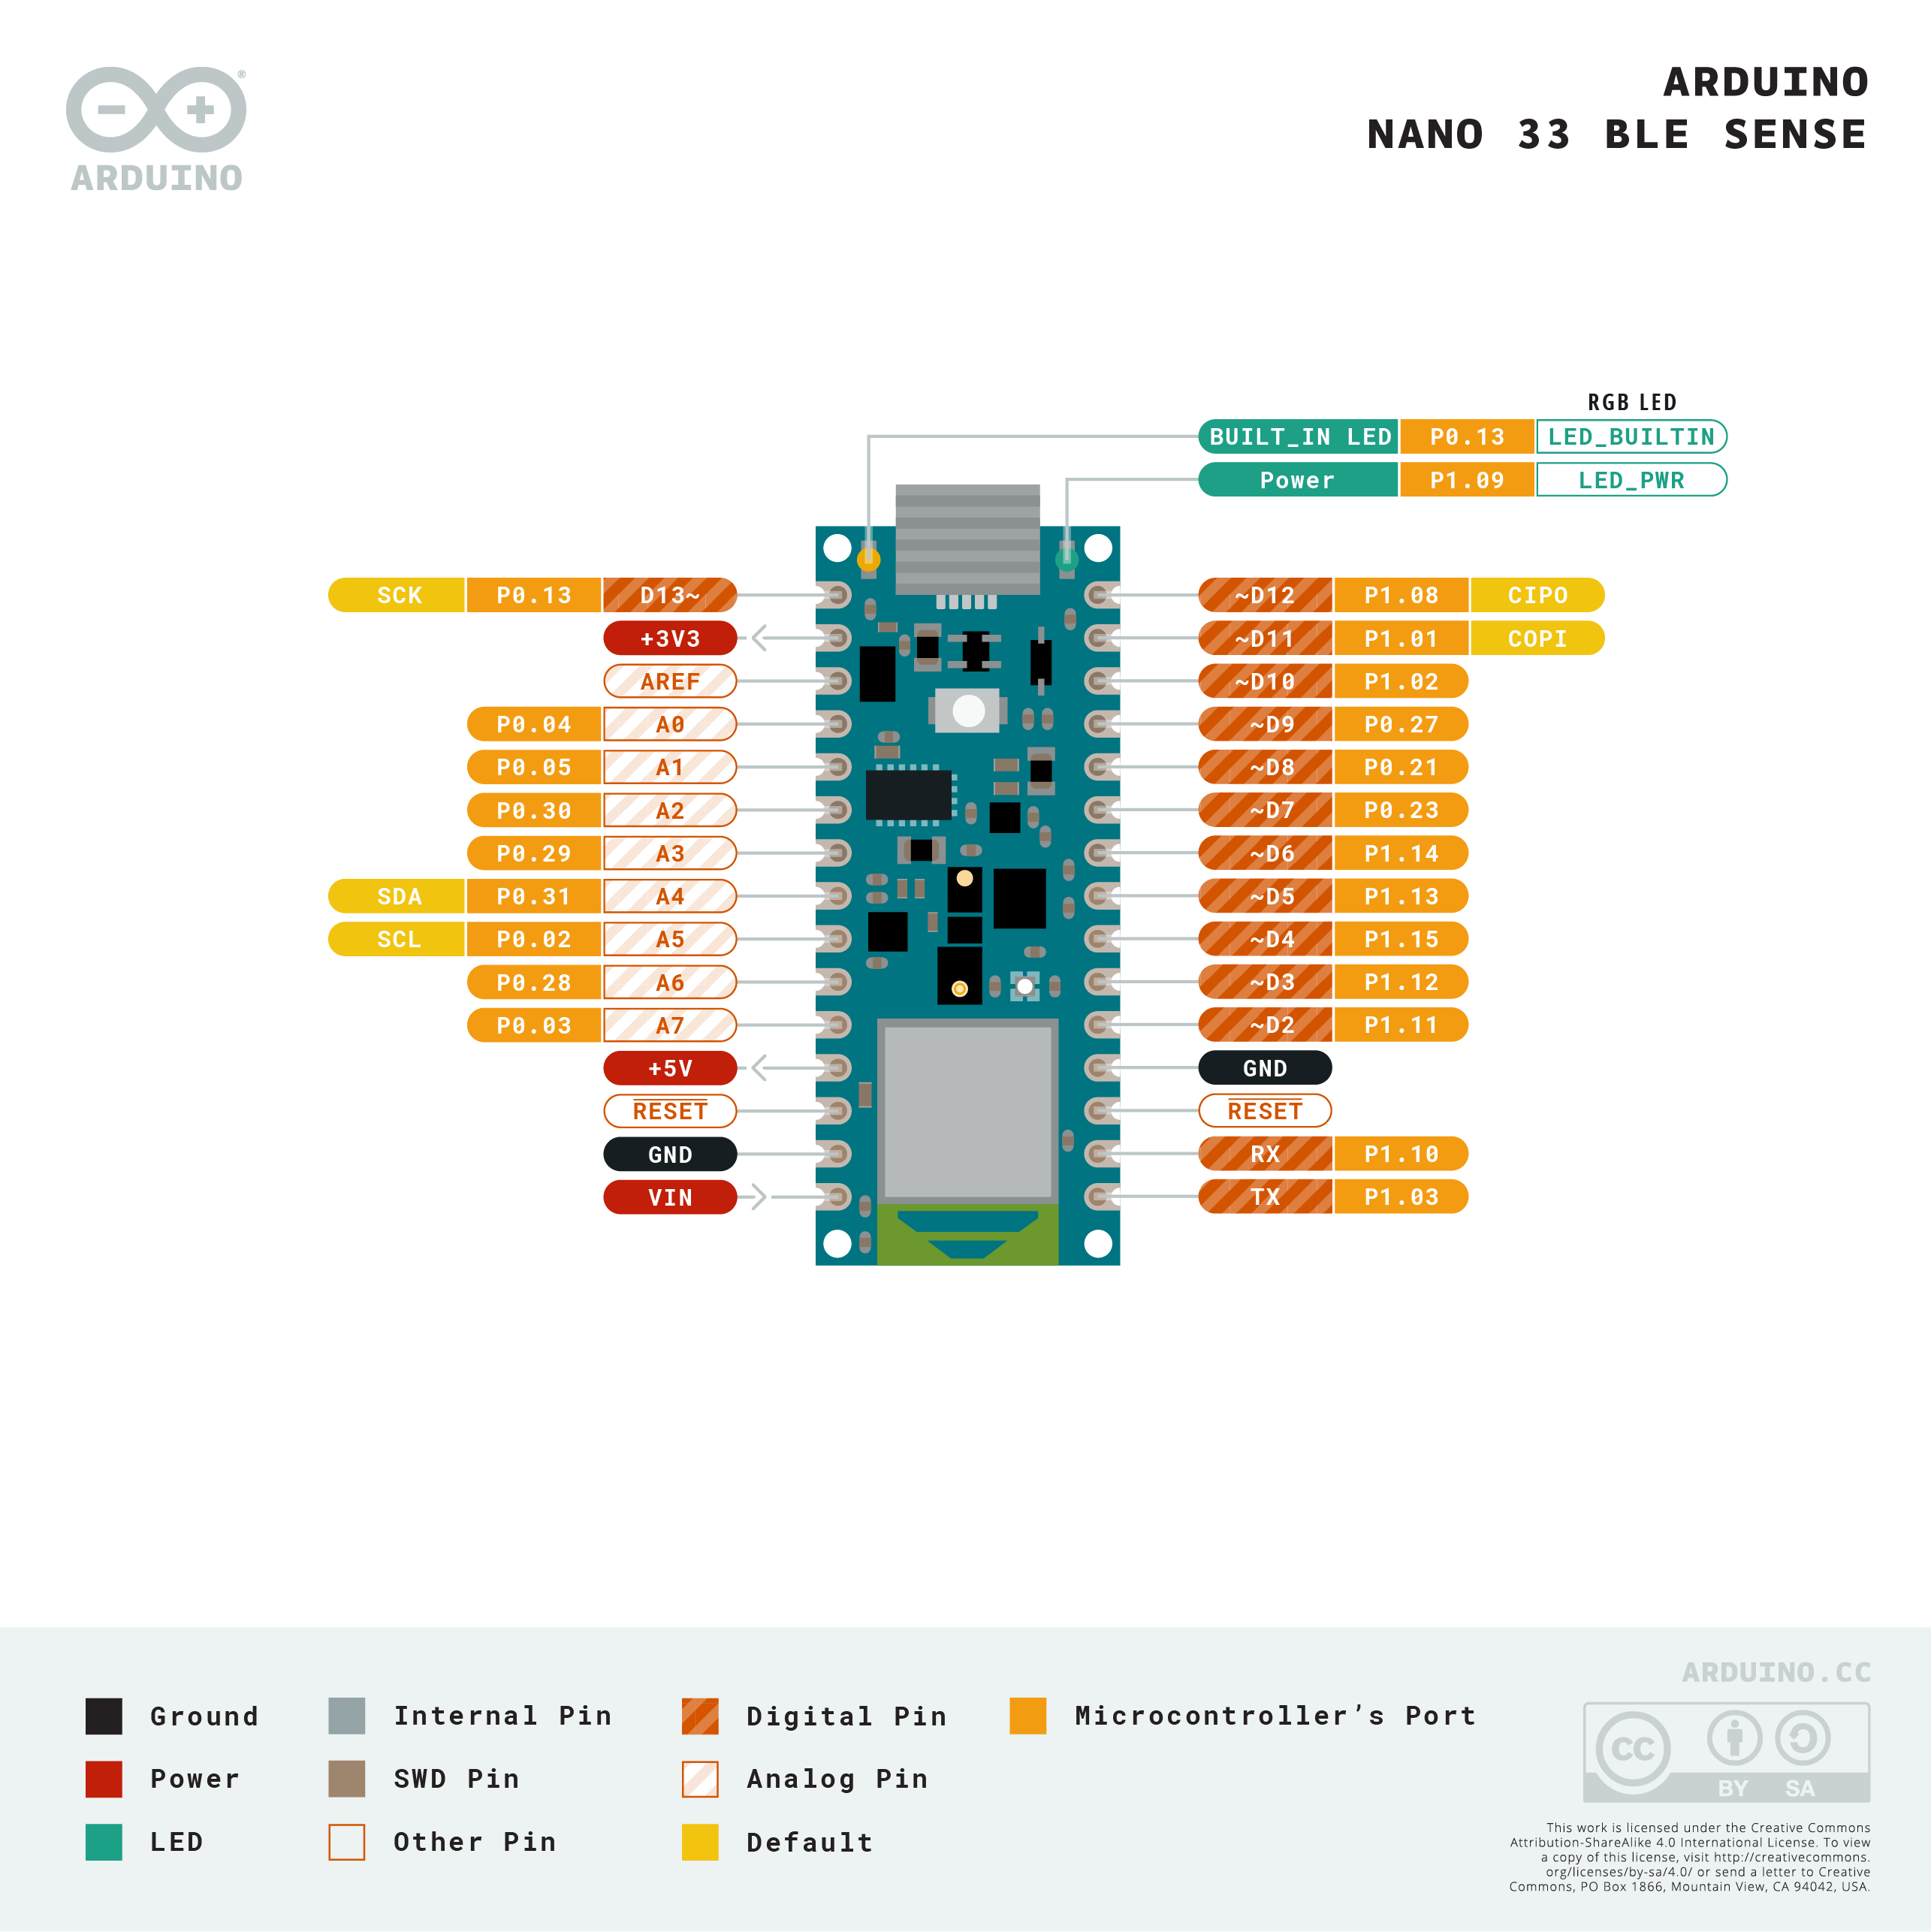
\includegraphics[scale=0.7]{./images/io.png} 
\caption{Diagrama de pines \cite{placa}}
\label{f2}
\end{figure}

\begin{figure}[H]
\centering
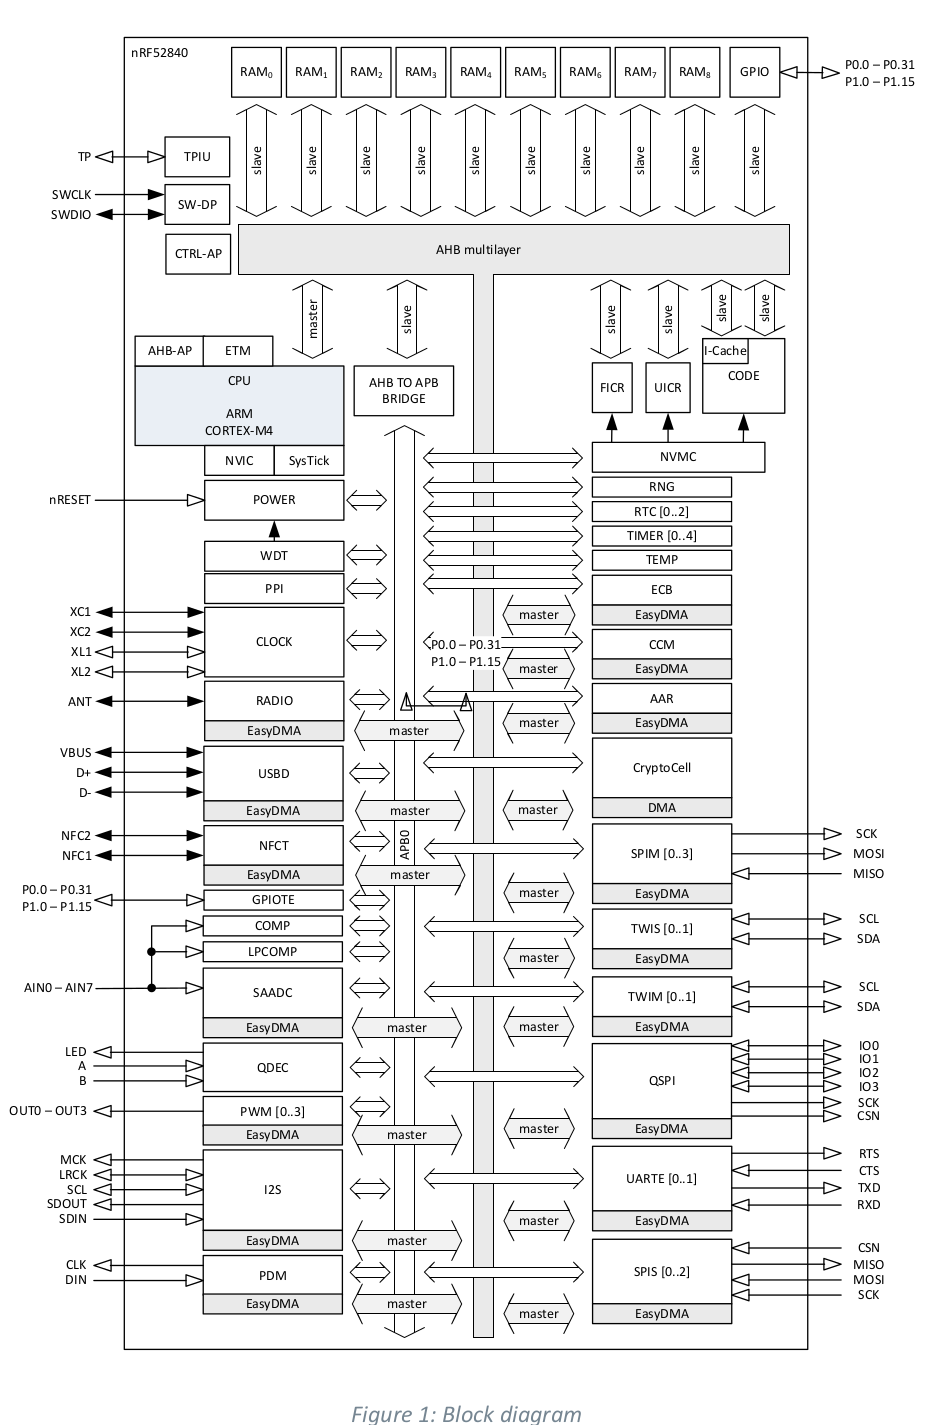
\includegraphics[scale=0.6]{./images/bloques.png} 
\caption{Diagrama de bloques \cite{mcu}}.
\label{f3}
\end{figure}

\subsection{Sobre el Nano 33 BLE Sense}

El Arduino Nano 33 BLE Sense es una excelente opción para cualquier principiante, fabricante o profesional para comenzar con el aprendizaje automático integrado. Se basa en el microcontrolador nRF52840 y se ejecuta en el sistema operativo Arm Mbed. El Nano 33 BLE Sense no solo cuenta con la posibilidad de conectarse a través de Bluetooth Low Energy, sino que también viene equipado con sensores para detectar color, proximidad, movimiento, temperatura, humedad, audio y más \cite{placa}.\\
Sobre sus periféricos y principales características:
\begin{itemize}
    \item \textbf{u-blox NINA-B306:} Módulo Bluetooth 5 de bajo consumo de u-blox, con antena interna \cite{placa}.
    \item \textbf{IMU for Motion Detection:} La unidad de medición inercial LSM9DS1 cuenta con un acelerómetro, un giroscopio y un magnetómetro 3D y le permite detectar la orientación, el movimiento o las vibraciones en su proyecto \cite{placa}. Se trata de un sistema en paquete que presenta un sensor de aceleración lineal digital 3D, un sensor digital 3D, un sensor de velocidad angular y un sensor magnético digital 3D \cite{acele}.
    
    
    \begin{itemize}
        \item  3 canales de aceleración, 3 de velocidad angular canales, 3 canales de campo magnético \cite{acele}.
        \item Interfaces seriales SPI / $I^2C$ \cite{acele}.
        \item 16-bit de data-output \cite{acele}.
    \end{itemize}
    \item \textbf{Omnidirectional Digital Microphone:} El micrófono MP34DT05 permite capturar y analizar el sonido en tiempo real y puede usarse para crear una interfaz de voz para su proyecto\cite{placa}.
    \item \textbf{Proximity and Gesture Detection:} El chip APDS-9960 permite medir la proximidad digital y la luz ambiental, así como detectar colores y gestos RGB \cite{placa}.
    \item \textbf{Barometric Pressure Sensor:} El LPS22HB detecta la presión barométrica y permite una salida de datos de presión de 24 bits entre 260 y 1260 hPa. Estos datos también se pueden procesar para calcular la altura sobre el nivel del mar de la ubicación actual \cite{placa}.
    \item \textbf{Temperature and Humidity Detection: }The HTS221 capacitive digital sensor measures relative humidity and temperature. It has a temperature accuracy of ± 0.5 °C (between 15-40 °C) and is thereby perfectly suited to detect ambient temperature \cite{placa}.






\end{itemize}




